%!TEX root = main.tex

\section{Screened dual of Sinkhorn divergence} % (fold)
\label{sec:screened_dual_of_sinkhorn_divergence}

\begin{wrapfigure}{o}{0.44\textwidth}
\vspace{-15pt}
\centering
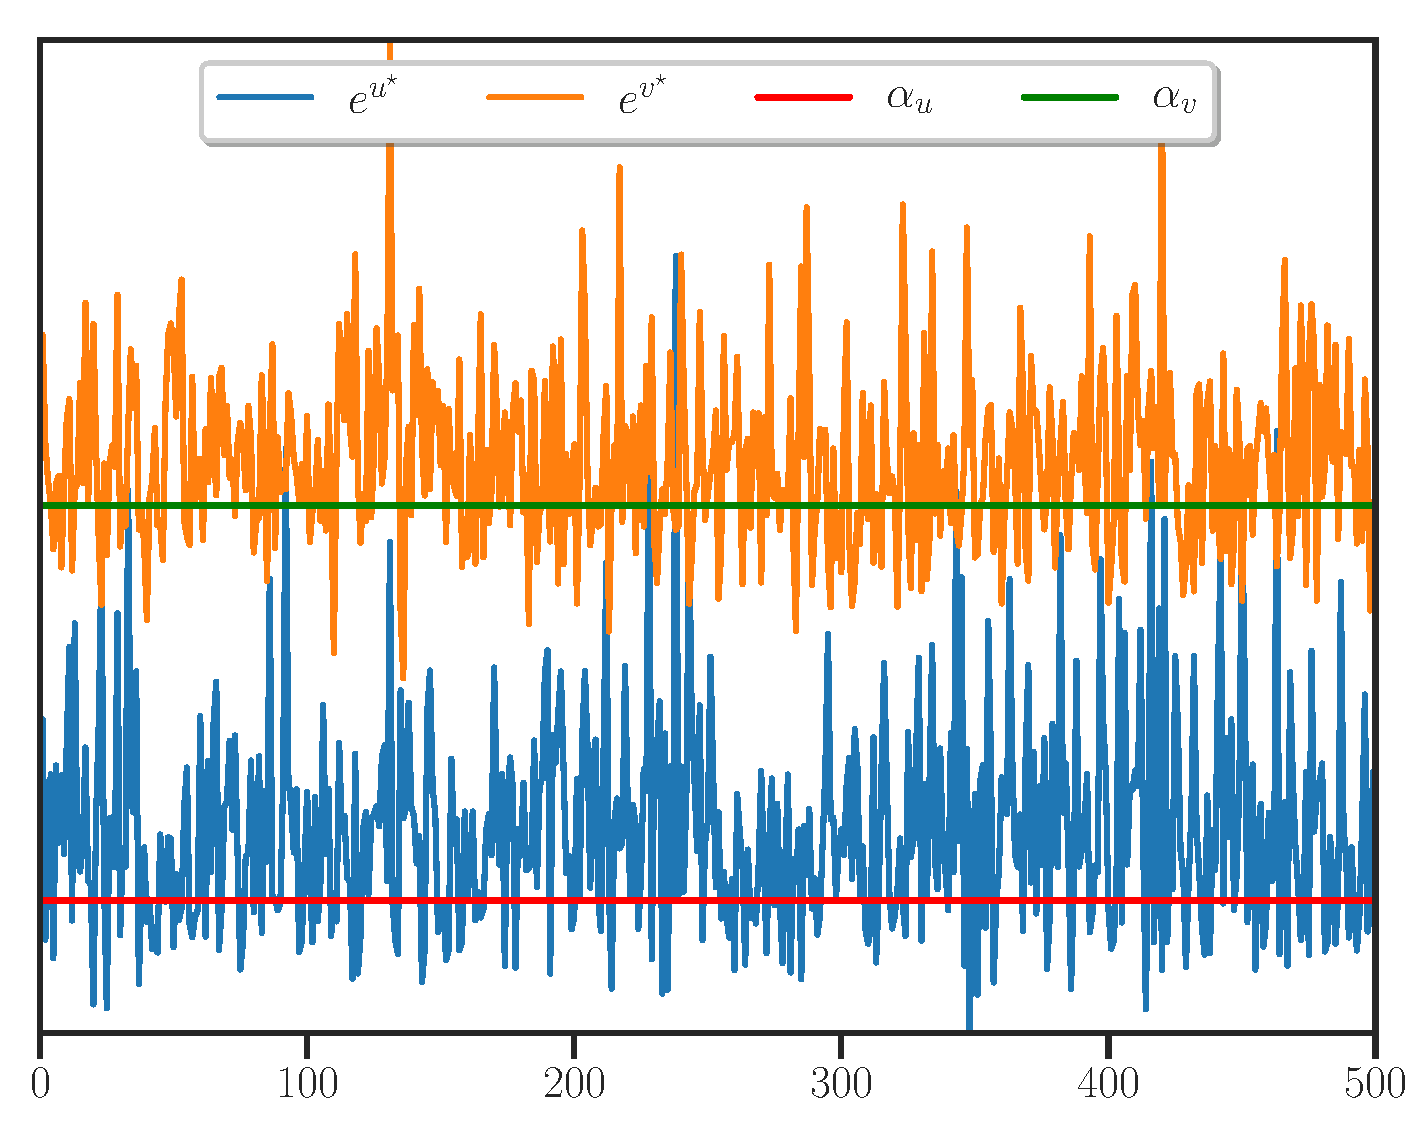
\includegraphics[width=0.45\textwidth]{./figs/motivations.pdf}
\caption{Plots of $(e^{u^\star}, e^{v^\star})$ with $(u^\star, v^\star)$ is the pair solution of dual of Sinkhorn divergence~\ref{sinkhorn-dual} and the thresholds $\alpha_u, \alpha_v$.}
\label{fig:motivations}
\vspace{-11pt}
\end{wrapfigure}

\paragraph{Motivation.} 

The key idea of our approach is motivated by the so-called \emph{static screening test}~\citep{Ghaoui2010SafeFE} in supervised learning, which is a method able to quickly identify inactive features, i.e., features that have zero components in the solution vector. 
Then, these inactive features can be removed from the optimization problem to reduce its scale.
Before diving into detailed algorithmic analysis, let's us present a brief illustration of how we adapt static screening test to the dual of Sinkhorn divergence.
Towards this end, we define the convex set $\mathcal{C}^r_{\alpha} \subseteq \R^r$, for $r\in \mathbb N$ and $\alpha >0$, by $\mathcal{C}^r_{\alpha} = \{w\in \R^{r}: \min_{1\leq i\leq r} e^{w_i} \geq \alpha\}$.
In Figure~\ref{fig:motivations}, we plot $(e^{u^\star}, e^{v^\star})$ where $(u^\star, v^\star)$ is the pair solution of dual of Sinkhorn divergence~(\ref{sinkhorn-dual}) in the particular case of: $n=m=500, \eta=0.1, \mu = \nu = \frac 1n \mathbf 1_n$ and the cost matrix $C$ corresponds the pairwise euclidean distance, i.e., $C_{ij} = \norm{x_i - y_j}_2$. 
We also plot two lines corresponding to $e^{u^\star} \equiv \alpha_u$ and $e^{v^\star} \equiv \alpha_v$ for some $\alpha_u>0$ and $\alpha_v >0$, playing the role of thresholds to select indices to be discard from the optimization procedure.

\paragraph{Static screening test.} The core of the static screening test developed in this paper aims at locating two subsets of indices $(I, J)$ in $\{1, \ldots, n\}\times\{1, \ldots, m\}$ satisfying: $e^{u_i}\geq \alpha_u, \text{ and } e^{v_j}\geq \alpha_v, \text{ for all } (i,j) \in I \times J$ and 
$e^{u_{i'}} = \alpha_u, \text{ and } e^{v_{j'}} = \alpha_v, \text{ for all } (i',j') \in I^\complement \times J^\complement$, namely $(u,v) \in \mathcal{C}^n_{\alpha_u}\times \mathcal{C}^m_{\alpha_v}$.
The sets $I$ and $J$ are called active sets, we further emphasize that they are determined in an initialization step in the proposed algorithm before running the L-BFGS-B solver.
Consequently, we can work on a "screened" dual of Sinkhorn divergence by considering variables that belong only to $\R^{|I|} \times \R^{|J|}$ in order to reduce the computational cost.

In the following, the parameters $\alpha_u = \varepsilon \kappa^{-1}$ and $\alpha_v = \varepsilon \kappa$ where $\varepsilon > 0$ and $\kappa > 0$ are fixed numeric constants to be given later. 
Our screening test relies on a new formulation of problem~\eqref{sinkhorn-dual}, that we refer as to \emph{approximate dual of Sinkhorn divergence}, defined by:

\begin{equation} 
\label{screen-sinkhorn}
\min_{u \in \mathcal{C}^n_{\frac \varepsilon \kappa}, v\in \mathcal{C}^m_{\varepsilon\kappa}} \big\{\Psi_{\kappa}(u,v):= \mathbf{1}_n^\top B(u,v)\mathbf{1}_m - \inr{\kappa u, \mu} - \inr{\frac v\kappa, \nu} \big\},
\end{equation}
The $\kappa$-parameter plays a role of scaling factor, allowing to get a closed order of the potential components $e^u$ and $e^v$, while the $\varepsilon$-parameter acts like a threshold for these components.
Note that the approximate dual of Sinkhorn divergence coincides with the dual of Sinkhorn divergence~\eqref{sinkhorn-dual} in the setting of $\varepsilon=0$ and $\kappa=1$.
As explained above, our static screening test is based on constructing two {active sets} denoted $I_{\varepsilon, \kappa}$ and $J_{\varepsilon, \kappa}$ throughout the dual problem of~\eqref{screen-sinkhorn} as follows: 

\begin{lemma}
\label{lemma_actives_sets}
Let $(u^{*}, v^{*})$ be an optimal solution of problem~\eqref{screen-sinkhorn}. 
Define
\begin{equation}
\label{I_epsilon_kappa_J_epsilon_kappa}
I_{\varepsilon,\kappa} = \big\{i=1, \ldots, n: \mu_i \geq \frac {\varepsilon^2} \kappa^{} r_i(K)\big\}, J_{\varepsilon,\kappa} = \big\{j=1, \ldots, m: \nu_j \geq \kappa{\varepsilon^2}{} c_j(K)\big\}
\end{equation}
Then one has $e^{u^{*}_i} = \varepsilon\kappa^{-1}$ and $e^{v^{*}_j} = \varepsilon\kappa$ for all $i \in I^\complement_{\varepsilon,\kappa} $ and $j\in J^\complement_{\varepsilon,\kappa} .$
\end{lemma}

Proof of Lemma~\ref{lemma_actives_sets} is postponed to the supplementary material. It is worth to note that first order optimality conditions applied to $(u^{*}, v^{*})$ ensure that if $e^{u^{*}_i} > \varepsilon\kappa^{-1}$ then $e^{u^{*}_i} (Ke^{v^{*}})_i =  \kappa\mu_i$ and if $e^{v^{*}_j} > \varepsilon\kappa$ then $e^{v^{*}_j} (K^\top e^{u^{*}})_j =  \kappa^{-1}\nu_j$, that correspond to the Sinkhorn marginal conditions~\citep{peyre2019COTnowpublisher} up to the scaling factor $\kappa$. 

\paragraph{Screening with a fixed number budget of points.}

Recall that the approximate dual of Sinkhorn divergence is defined with respect to $\varepsilon$ and $\kappa$, where its values depend on a priori \emph{fixed number budget of points} from the supports of $\mu$ and $\nu$.
In the sequel, we denote by $n_b \in\{1, \ldots, n\}$ and $m_b\in\{1, \ldots, m\}$ the number budget of points to be given for resolving problem~\eqref{screen-sinkhorn}. More precisely, we change the domain of the objective function $\Psi_\kappa$ from $\R^n \times \R^m$ to $\R^{n_b} \times \R^{m_b}$.

\begin{wrapfigure}{o}{0.44\textwidth}
\vspace{-18pt}
\centering
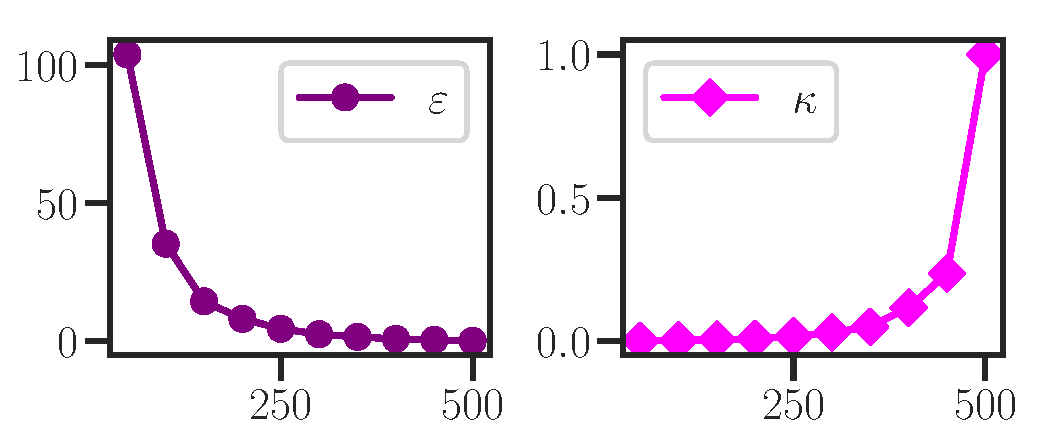
\includegraphics[width=0.46\textwidth]{./figs/kappa_epsilon.pdf}
\caption{Plots of $\varepsilon$ and $\kappa$ as a function of number budget of points for a screening test with $n_b=m_b$ and the parameters $\mu, \nu, \eta, C$ are set as in Figure~\eqref{fig:motivations}.  $(\varepsilon, \kappa)$ tends to $(0,1)$ as $(n_b,m_b)$ tends to $(n,m)$.}
\label{fig:kappa_epsilon}
\vspace{-15pt}
\end{wrapfigure}

In this spirit, let us define $\xi \in \R^n$ and $\zeta \in \R^m$ to be the ordered decreasing vectors of $\mu \oslash r(K)$ and $\nu \oslash c(K)$ respectively, that is $\xi_1 \geq \xi_2 \geq \cdots \geq \xi_n$ and $\zeta_1 \geq \zeta_2 \geq \cdots \geq \zeta_m$.
To keep only $n_b$-budget and $m_b$-budget of points, the parameters $\kappa$ and $\varepsilon$ satisfy ${\varepsilon^2}\kappa^{-1} = \xi_{n_b}$ and $\varepsilon^2\kappa = \zeta_{m_b}$. Hence 
\begin{equation}
\label{epsilon_kappa}
 \varepsilon = (\xi_{n_b}\zeta_{m_b})^{1/4} \text{ and } \kappa = \sqrt{\frac{\zeta_{m_b}}{\xi_{n_b}}}.
\end{equation}
Note that in one hand we have $|I_{\varepsilon, \kappa}| = n_b$ and $|J_{\varepsilon, \kappa}| = m_b$ by construction. On the other hand, when $(n_b,m_b)$ tends to the full number budget of points $(n,m)$, the couple parameters $(\varepsilon, \kappa)$ converges to $(0,1)$. 
In Figure~\ref{fig:kappa_epsilon}, we plot these convergences, and hence the objective in problem \eqref{screen-sinkhorn} converges to the objective of dual of Sinkhorn divergence~\eqref{sinkhorn-dual}.

Using the previous analysis, any solution $(u^*, v^*)$ of problem~\eqref{screen-sinkhorn} satisfies $e^{u^*_i} \geq \varepsilon\kappa^{-1}$ and $e^{v^*_j} \geq \varepsilon\kappa$ for all $(i,j) \in (I_{\varepsilon,\kappa}\times J_{\varepsilon,\kappa}),$ and $e^{u^*_i} = \varepsilon\kappa^{-1}$ and $e^{v^*_j} = \varepsilon\kappa$ for all $(i,j) \in (I^\complement_{\varepsilon,\kappa}\times J^\complement_{\varepsilon,\kappa})$.
Basing on that facts we restrict the constraints feasibility $\mathcal{C}^n_{\frac \varepsilon \kappa} \cap \mathcal{C}^m_{\varepsilon\kappa}$ to the screened domain defined by $\mathcal{U}_{\text{sc}} \cap \mathcal{V}_{\text{sc}}$, 
\begin{equation*}
\mathcal{U}_{\text{sc}} = \{u \in \R^{n_b}: e^{u_{I_{\varepsilon,\kappa}}} \succeq \frac \varepsilon\kappa\mathbf 1_{n_b}\} \text{ and } \mathcal{V}_{\text{sc}} =\{v\in\R^{m_b}: e^{v_{J_{\varepsilon,\kappa}}} \succeq \varepsilon\kappa \mathbf{1}_{m_b}\}%, \text{ and } e^{u_{I^\complement_{\varepsilon,\kappa}}} = \frac\varepsilon\kappa\mathbf 1_{n - n_b}\},
\end{equation*}
% and 
% \begin{equation*}
% 	\mathcal{V}_{\text{sc}} =\{v\in\R^m: e^{v_{J_{\varepsilon,\kappa}}} \succeq \varepsilon\kappa \mathbf{1}_{m_b}\}. %, \text{ and } e^{v_{J^\complement_{\varepsilon,\kappa}}} = \varepsilon\kappa \mathbf 1_{m- m_b}\}.
% \end{equation*}
where the vector comparison $\succeq$ has to be understood elementwise.
Now, we are ready to define the \emph{screened dual of Sinkhorn divergence} as
\begin{align}
\label{screen-sinkhorn_second_def}
\min_{u \in \mathcal{U}_{\text{sc}}, v \in \mathcal{V}_{\text{sc}}}\{\Psi_{\varepsilon, \kappa}(u,v)\}
\end{align}
where 
\begin{align*} 
\Psi_{\varepsilon,\kappa}(u, v) &= (e^{u_{I_{\varepsilon,\kappa}}})^\top K_{(I_{\varepsilon,\kappa}, J_{\varepsilon,\kappa})} e^{v_{J_{\varepsilon,\kappa}}} + 
\varepsilon \kappa (e^{u_{I_{\varepsilon,\kappa}}})^\top K_{(I_{\varepsilon,\kappa}, J^\complement_{\varepsilon,\kappa})}\mathbf 1_{m_b} + \varepsilon \kappa^{-1} \mathbf 1_{n_b}^\top K_{(I^\complement_{\varepsilon,\kappa}, J_{\varepsilon,\kappa})}e^{v_{J_{\varepsilon,\kappa}}}\\
&\qquad - \kappa \mu_{I_{\varepsilon,\kappa}}^\top u_{I_{\varepsilon,\kappa}} - \kappa^{-1} \nu_{J_{\varepsilon,\kappa}}^\top v_{J_{\varepsilon,\kappa}} + \Xi
\end{align*}
with $\Xi = \varepsilon^2 \sum_{i \in I^\complement_{\varepsilon,\kappa}, j \in J^\complement_{\varepsilon,\kappa}} K_{ij} -\kappa \log(\varepsilon\kappa^{-1})\sum_{i \in I^\complement_{\varepsilon,\kappa}}\mu_i - \kappa^{-1} \log(\varepsilon\kappa)\sum_{j\in J^\complement_{\varepsilon,\kappa}} \nu_j$.

Pseudocode of our proposed algorithm is shown in Algorithm~\ref{screenkhorn}. %~\cite{nocedal1980,nocedal2006numerical}
It is worth to note that \emph{Screenkhorn} algorithm uses only the restricted parts $K_{(I_{\varepsilon,\kappa}, J_{\varepsilon,\kappa})},$ $K_{(I_{\varepsilon,\kappa}, J^\complement_{\varepsilon,\kappa})},$ and $K_{(I^\complement_{\varepsilon,\kappa}, J_{\varepsilon,\kappa})}$ of the Gibbs kernel $K$ for calculating the objective function $\Psi_{\varepsilon, \kappa}$ and its gradient, in contrast to Sinkhorn algorithm which performs alternating updates of all rows and columns of $K.$
Furthermore, \emph{Screenkhorn} consists of two steps: the first one is an initialization providing the active sets $I_{\varepsilon,\kappa}$, $J_{\varepsilon,\kappa}$. 
The second is a constrained L-BFGS-B for the stacked variable $\theta=(u_{I_{\varepsilon,\kappa}},v_{J_{\varepsilon,\kappa}}).$ 
L-BFGS-B handles box constraints on variables, and it becomes more efficient when these box bounds are carefully determined for problem~\eqref{screen-sinkhorn_second_def}. 
The following proposition (proof in supplementary material) expresses these bounds that are pre-calculated in the initialization step of \emph{Screenkhorn}.
\begin{proposition}
\label{prop:bounds_of_usc_and_vsc}
Let $(u^{\text{sc}}, v^{\text{sc}})$ be an optimal pair solution of problem~\eqref{screen-sinkhorn_second_def} and $K_{\min} = \min\limits_{i\in I_{\varepsilon,\kappa},j \in J_{\varepsilon,\kappa}}K_{ij}$. Then,
one has
\begin{equation}
\label{bound_on_u}
\frac \varepsilon\kappa \vee \frac{\min_{i \in I_{\varepsilon,\kappa}}\mu_i}{\varepsilon (m- m_b) + \varepsilon \vee \frac{\max_{j\in J_{\varepsilon,\kappa}} \nu_j}{n\varepsilon\kappa K_{\min}} m_b} \leq e^{u^{\text{sc}}_i} \leq \frac \varepsilon\kappa\vee \frac{\max_{i \in I_{\varepsilon,\kappa}} \mu_i}{m\varepsilon K_{\min}},
\end{equation}
and
\begin{equation}
\label{bound_on_v}
\varepsilon\kappa \vee \frac{\min_{j \in J_{\varepsilon,\kappa}}\nu_j}{\varepsilon(n- n_b) + \varepsilon \vee \frac{\kappa\max_{i\in I_{\varepsilon,\kappa}} \mu_i}{m\varepsilon K_{\min} } n_b} \leq e^{v^{\text{sc}}_j} \leq \varepsilon\kappa \vee \frac{\max_{j \in J_{\varepsilon,\kappa}} \nu_j}{n\varepsilon K_{\min} }
\end{equation}
for all $i\in I_{\varepsilon,\kappa}$ and $j\in J_{\varepsilon,\kappa}$.
\end{proposition}
\LinesNotNumbered
\begin{algorithm}[htbp]
\SetNlSty{textbf}{}{.}
\DontPrintSemicolon
\caption{\emph{Screenkhorn}$(C,\eta,\mu,\nu,n_b,m_b)$}
\label{screenkhorn}

\textbf{Step 1:} \textcolor{black}{Initialization}\\

\nl   $\xi \gets \texttt{sort}(\mu \oslash r(K)),$ $\zeta \gets \texttt{sort}(\nu \oslash c(K));$ //(decreasing order)\\
% \nl   $\zeta \gets \texttt{sort}(\nu \oslash c(K));$\\
% \nl   $\xi \gets \texttt{sort}(\xi);$ //(decreasing order)\\
% \nl   $\zeta \gets \texttt{sort}(\zeta);$ //(decreasing order)\\
\nl   $\varepsilon \gets (\xi_{n_b}\zeta_{m_b})^{1/4}, \text{  } \kappa \gets \sqrt{{\zeta_{m_b}}/{\xi_{n_b}}}$;\\
\nl   $I_{\varepsilon,\kappa} \gets \{i=1, \ldots, n: \mu_i \geq {\varepsilon^2} \kappa^{-1} r_i(K)\};$\\
\nl   $J_{\varepsilon,\kappa} \gets \{j=1, \ldots, m: \nu_j \geq \varepsilon^2\kappa c_j(K)\};$\\ 
\nl   $\underline{\mu} \gets \min_{i \in I_{\varepsilon,\kappa}} \mu_i, \bar{\mu} \gets \max_{i \in I_{\varepsilon,\kappa}} \mu_i$; \\
\nl   $\underline{\nu} \gets \min_{j \in J_{\varepsilon,\kappa}} \mu_i, \bar{\nu} \gets \max_{j \in J_{\varepsilon,\kappa}} \mu_i$; \\
\nl   $\underline{u} \gets \log\big(\frac \varepsilon\kappa \vee \frac{\underline{\mu}}{\varepsilon (m-m_b) + \varepsilon \vee \frac{\bar{\nu}}{n\varepsilon\kappa K_{\min}} m_b}\big), \bar{u} \gets  \log\big(\frac \varepsilon\kappa\vee \frac{\bar{\mu}}{m\varepsilon K_{\min}}\big);$\\
\nl   $\underline{v} \gets \log\big(\varepsilon\kappa \vee \frac{\underline{\nu}}{\varepsilon(n-n_b) + \varepsilon \vee \frac{\kappa\bar{\mu}}{m\varepsilon K_{\min}} n_b}\big), \bar{v} \gets \log\big(\varepsilon\kappa \vee \frac{\bar{\nu}}{n\varepsilon K_{\min}}\big);$\\
\nl   $ \bar{\theta} \gets \texttt{stack}(\bar{u}\mathbf 1_{n_b}, \bar{v}\mathbf 1_{m_b}),$ $ \underline{\theta} \gets \texttt{stack}(\underline{u}\mathbf 1_{n_b}, \underline{v}\mathbf 1_{m_b}) ;$\\
% \nl   $ \underline{\theta} \gets \texttt{stack}(\underline{u}\mathbf 1_{n_b}, \underline{v}\mathbf 1_{m_b}) ;$\\

\noindent \textbf{Step 2:} \textcolor{black}{L-BFGS-B}\\

\nl  $u^{(0)}\gets \log(\varepsilon\kappa^{-1}) \mathbf 1_{n_b},$ $v^{(0)} \gets \log(\varepsilon\kappa) \mathbf 1_{m_b},$ $\theta^{(0)} \gets \texttt{stack}(u^{(0)}, v^{(0)});$\\
% \nl  $v^{(0)} \gets \log(\varepsilon\kappa) \mathbf 1_{m_b} ;$\\
% \nl  $\theta^{(0)} \gets \texttt{stack}(u^{(0)}, v^{(0)});$\\
\nl   $\theta \gets \text{L-BFGS-B}(\theta^{(0)}, \underline{\theta}, \bar{\theta});$\\
\nl   $\theta_u \gets (\theta_1, \ldots, \theta_{n_b})^\top, \theta_v \gets(\theta_{n_b+1}, \ldots, \theta_{n_b+m_b})^\top;$\\
\nl   {$u^{sc}_i \gets (\theta_u)_i$ if $i \in I_{\varepsilon,\kappa}$ and $u_i \gets \log(\varepsilon\kappa^{-1})$ if $i \in I^\complement_{\varepsilon,\kappa};$}\\
\nl   {$v^{sc}_j \gets (\theta_v)_j$ if $j \in J_{\varepsilon,\kappa}$ and $v_j \gets \log(\varepsilon\kappa)$ if $j \in J^\complement_{\varepsilon,\kappa};$}\\
\nl   \Return{$B(u^{\text{sc}},v^{\text{sc}})$.}
\end{algorithm}

% section screened_dual_of_sinkhorn_divergence (end)